\marginfigeometry

\section{START-UP}

\subsection{PRE-START}
\begin{checklistenumerate}
    \blueitem[Verify Check]\cbstart
    \marcautionbox{
        \small\textbf{Failure to verify switch position can lead to major system malfunction during start-up}
    }
    \begin{enumerate}
        \item \textbf{FUEL MASTER Switch} \dotfill \textbf{MASTER}
        \item \textbf{ENG FEED Knob} \dotfill \textbf{NORM}
        \item \textbf{EPU Switch} \dotfill \textbf{NORM}
        \item \textbf{ENG CONT Switch} \dotfill \textbf{PRI}
        \item \textbf{Throttle} \dotfill \textbf{OFF}
        \item \textbf{LG Handle} \dotfill \textbf{DN}
        \item \textbf{HOOK Switch} \dotfill \textbf{UP}
        \item \textbf{MASTER ARM Switch} \dotfill \textbf{OFF}
        \item \textbf{AIR SOURCE Knob} \dotfill \textbf{NORM}
    \end{enumerate}
    \cbend
    \blueitem[{\hyperref[fig:proc_basic:prestart:flcscheck]{FLCS Check}}]
    \marginpar{
        \captionsetup{type=figure}
        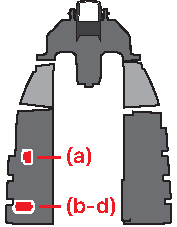
\includegraphics[width=\marginparwidth]{diagrams/cockpit/flcs_check.pdf}
        \caption{FLCS Check}
        \label{fig:proc_basic:prestart:flcscheck}
    }
    \begin{enumerate}
        \item \textbf{Main PWR Switch}\cbstart \dotfill \textbf{BATT}\cbend
        \begin{itemize}
            \item \textbf{FLCS RLY Light} --- \textbf{ON}
        \end{itemize}
        \item \textbf{FLCS PWR TEST} \dotfill \textbf{TEST (hold)}
        \item \textbf{Test Lights} \dotfill \textbf{Verify}
        \begin{itemize}
            \item \textbf{ACFT BATT TO FLCS} --- \textbf{ON}
            \item \textbf{FLCS PMG} --- \textbf{ON}
            \item \textbf{FLCS PWR} --- \textbf{ON}
            \item \textbf{FLCS RLY} --- \textbf{OFF}
        \end{itemize}
        \item \textbf{FLCS PWR TEST} \dotfill \textbf{Release}
    \end{enumerate}
    \blueitem[{\hyperref[fig:proc_basic:prestart:mainpower]{Main Power}}]
    \marginpar{
        \captionsetup{type=figure}
        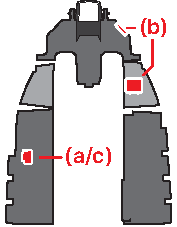
\includegraphics[width=\marginparwidth]{diagrams/cockpit/main_power.pdf}
        \caption{Main Power}
        \label{fig:proc_basic:prestart:mainpower}
    }
    \begin{enumerate}
        \item \textbf{Main PWR Switch}\cbstart \dotfill \textbf{MAIN}\cbend
        \item \textbf{Warning Lights} \dotfill \textbf{Check}
        \begin{itemize}
            \item \textbf{ELEC SYS} --- \textbf{ON}
            \item \textbf{HYD/OIL PRESS} --- \textbf{ON}
            \item \textbf{FLCS RLY} --- \textbf{ON}
            \item \textbf{SEC} --- \textbf{ON}
            \item \textbf{ENGINE} --- \textbf{ON}
        \end{itemize}
        \item \textbf{EPU Lights} \dotfill \textbf{Confirm OFF}
        \begin{itemize}
            \item \textbf{EPU GEN Light} --- \textbf{OFF}
            \item \textbf{EPU PMG Light} --- \textbf{OFF}
        \end{itemize}
    \end{enumerate}
\end{checklistenumerate}

\clearpage

\subsection{ENGINE START}
\begin{checklistenumerate}
    \blueitem[Engine Start]\cbstart
    \marginpar{
        \captionsetup{type=figure}
        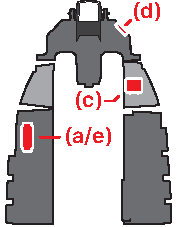
\includegraphics[width=\marginparwidth]{diagrams/cockpit/engine_start.pdf}
        \caption{Engine Start}
    }
    \begin{enumerate}
        \item \textbf{JFS Switch} \dotfill \textbf{START 2}
        \item \textbf{Throttle} \dotfill \textbf{IDLE} \\
        \hfill (once 20\% RPM reached)
        \item \textbf{SEC Light} \dotfill \textbf{OFF} 
        \item \textbf{ENGINE Warning Light} \dotfill \textbf{OFF} \\
        \hfill (once 60\% RPM reached)
        \item \textbf{JFS Switch} \dotfill \textbf{Confirm OFF}
    \end{enumerate}\cbend
    \blueitem[ENG Instruments]
    \marginpar{
        \captionsetup{type=figure}
        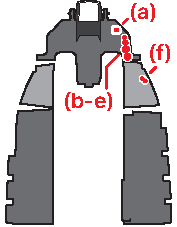
\includegraphics[width=\marginparwidth]{diagrams/cockpit/engine_instruments.pdf}
        \caption{ENG Instruments}
    }
    \begin{enumerate}
        \item \textbf{FUEL FLOW} --- 700-1700 PPH
        \item \textbf{OIL Pressure} --- 15 PSI (minimum)
        \item \textbf{NOZ POS} --- greater than 95\%
        \item \textbf{RPM} --- 62-80\% 
        \item \textbf{FTIT} --- 650C or less
        \item \textbf{HYD PRES A \& B} --- 2850-3250 PSI
    \end{enumerate}
\end{checklistenumerate}

\notebox{
    \textbf{Can close Canopy prior to advancing Throttle to IDLE to reduce cockpit noise}
}

\clearpage

\subsection{POST-START}
\begin{checklistenumerate}
    \blueitem[TEST Panel]
    \marginpar{
        \captionsetup{type=figure}
        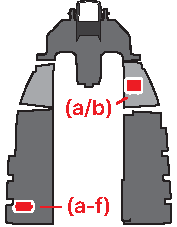
\includegraphics[width=\marginparwidth]{diagrams/cockpit/test_panel.pdf}
        \caption{TEST Panel}
    }
    \begin{enumerate}
        \item \textbf{PROBE HEAT Switch} \dotfill \textbf{PROBE HEAT} \\
        \hfill verify PROBE HEAT Caution Light --- off
        \item \textbf{PROBE HEAT Switch} \dotfill \textbf{TEST} \\
        \hfill verify PROBE HEAT C. Light --- flashing
        \item \textbf{PROBE HEAT Switch} \dotfill \textbf{OFF}
        \item \textbf{FIRE \& OHEAT DETECT} \dotfill \textbf{TEST}
        \item \textbf{OXY QTY Test Switch} \dotfill \textbf{TEST}
        \item \textbf{MAL \& IND LTS Button} \dotfill \textbf{TEST}
    \end{enumerate}
    \blueitem[AVIONICS Panel]\cbstart
    \marginpar{
        \captionsetup{type=figure}
        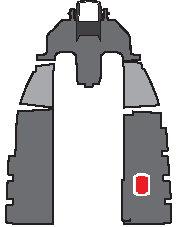
\includegraphics[width=\marginparwidth]{diagrams/cockpit/avionics_ins.pdf}
        \caption{Avionics \& INS}
    }
    \begin{enumerate}
        \item \textbf{MMC Switch} \dotfill \textbf{MMC}
        \item \textbf{ST STA Switch} \dotfill \textbf{ST STA}
        \item \textbf{MFD Switch} \dotfill \textbf{MFD}
        \item \textbf{UFC Switch} \dotfill \textbf{UFD}
        \item \textbf{GPS Switch} \dotfill \textbf{GPS}
        \item \textbf{DL Switch} \dotfill \textbf{DL}
        \item \textbf{MIDS LVT Knob} \dotfill \textbf{ON}
    \end{enumerate}
    \blueitem[INS Alignment]
    \begin{enumerate}
        \item \textbf{EGI/INS} \dotfill \textbf{Desired ALIGN Mode} \\
        \begin{itemize}
            \item \textbf{NORM} --- full align, approx. 8 min
            \item \textbf{STOR HDG} --- quick align, approx. 90 sec
        \end{itemize}
    \end{enumerate}
    \blueitem[SNSR PWR Panel]
    \marginpar{
        \captionsetup{type=figure}
        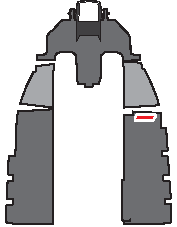
\includegraphics[width=\marginparwidth]{diagrams/cockpit/snsr_pwr.pdf}
        \caption{SNSR PWR Panel}
    }
    \begin{enumerate}
        \item \textbf{LEFT HDPT Switch} \dotfill \textbf{As Required} \\
        \hfill (if HTS pod installed)
        \item \textbf{RIGHT HDPT Switch} \dotfill \textbf{As Required} \\
        \hfill (if targeting pod installed)
        \item \textbf{FCR Switch} \dotfill \textbf{FCR}
        \item \textbf{RDR ALT Switch} \dotfill \textbf{RDR ALT}
    \end{enumerate}\cbend
\end{checklistenumerate}

\clearpage

\begin{checklistenumerate}[resume]
    \blueitem[HUD Setup]\cbstart
    \marginpar{
        \captionsetup{type=figure}
        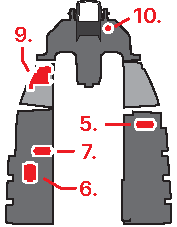
\includegraphics[width=\marginparwidth]{diagrams/cockpit/hud_sai.pdf}
        \caption{HUD, C\&I, ECM, SPD BRK, WHEELS Down, SAI}
    }
    \begin{enumerate}
        \item \textbf{HUD Control Panel} \dotfill \textbf{As Desired}
        \item \textbf{HUD Brightness} \dotfill \textbf{As Desired} 
    \end{enumerate}\cbend
    \blueitem[C\&I Knob]\dotfill\textbf{UFC}
    \blueitem[ECM Panel]\cbstart\dotfill\textbf{As Desired}\cbend
    \blueitem[SPD BRK Check]\dotfill\textbf{Cycle} (back to closed)
    \blueitem[WHEELS Down Lights]\dotfill Verify \textbf{Three Green}
    \blueitem[\cbstart  Standby Attitude Indicator\cbend]\dotfill\textbf{Set}
    \blueitem[Tests \& Checks]\dotfill\hyperref[subsec:testschecks]{\textbf{See \Cref{subsec:testschecks}}}
    \blueitem[Avionics Setup]
    \marginpar{%
        \captionsetup{type=figure}
        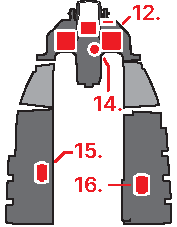
\includegraphics[width=\marginparwidth]{diagrams/cockpit/final_setup.pdf}
        \caption{Final Setup}
    }
    \cbstart\dotfill\textbf{Program As Required}
    \blueitem[Canopy]\dotfill\textbf{Close and Lock}
    \blueitem[Altimeter]\dotfill\textbf{Set and Check}
    \blueitem[Exterior Lights]\dotfill\textbf{As Desired}
    \blueitem[INS Knob]\dotfill\textbf{NAV}\cbend
    \blueitem[NWS]\dotfill\textbf{Engage}
    \blueitem[Throttle]\dotfill\textbf{Advance} (Check brakes \& NWS)
    \blueitem[Flight Instruments]\dotfill\textbf{Check}
\end{checklistenumerate}

% \clearpage

\cautionbox{
    \textbf{Do NOT rearm aircraft during INS align}
    \begin{itemize}
        \item Can interrupt INS alignment
        \item If interrupted recycle INS knob to off, then back to align
        \item Recommend rearming either before or after INS align
    \end{itemize}
}

\clearpage

\subsection{TESTS \& CHECKS}
\label{subsec:testschecks}
\begin{checklistenumerate}
    \blueitem[ENG SEC Mode]
    \marginpar{
        \captionsetup{type=figure}
        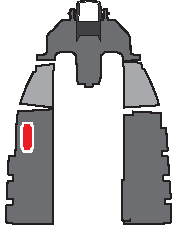
\includegraphics[width=\marginparwidth]{diagrams/cockpit/check_eng_sec.pdf}
        \caption{ENG SEC Mode}
    }
    \begin{enumerate}
        \item \textbf{ENG CONT Switch} \dotfill \textbf{SEC}
        \begin{itemize}
            \item \textbf{SEC Caution Light} --- \textbf{ON}
            \item \textbf{RPM} --- Stabilized
            \item \textbf{Throttle} --- Snap to \textbf{MIL}, then to \textbf{IDLE} when RPM reaches 85\% 
            \item \textbf{NOZ POS} --- < 10\% within 30s after \textbf{SEC} selection
        \end{itemize}
        \item \textbf{ENG CONT Switch} \dotfill \textbf{PRI}
        \begin{itemize}
            \item \textbf{SEC Caution Light} --- \textbf{OFF}
            \item \textbf{NOZ POS} --- > 94\% 
        \end{itemize}
    \end{enumerate}
    \blueitem[FLCS BIT]
    \marginpar{
        \captionsetup{type=figure}
        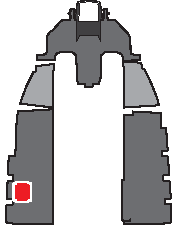
\includegraphics[width=\marginparwidth]{diagrams/cockpit/check_flcs_bit.pdf}
        \caption{FLCS BIT}
    }
    \begin{enumerate}
        \item \textbf{FLCS BIT Switch} \dotfill \textbf{BIT}
        \begin{itemize}
            \item \textbf{FLCP RUN Light} --- Illuminates
        \end{itemize}
        \item \textbf{BIT Completion}
        \begin{itemize}
            \item \textbf{Duration} --- Approx. 45s
            \item \textbf{FLCP RUN Light} --- Extinguishes
            \item \textbf{BIT Switch} --- Returns to \textbf{OFF}
            \item \textbf{FAIL Light} --- Verify \textbf{OFF}
            \item \textbf{FLCS Warning Light} --- Verify \textbf{OFF}
        \end{itemize}
    \end{enumerate}
\end{checklistenumerate}

\clearpage

\begin{checklistenumerate}[resume]
    \blueitem[FUEL QTY Check]
    \marginpar{
        \captionsetup{type=figure}
        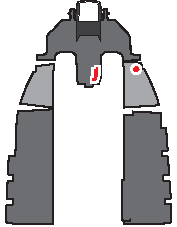
\includegraphics[width=\marginparwidth]{diagrams/cockpit/check_fuel_qty.pdf}
        \caption{FUEL QTY Check}
    }
    \begin{enumerate}
        \item \textbf{FUEL QTY SEL Knob} \dotfill \textbf{TEST}
        \begin{itemize}
            \item \textbf{FR/AL Pointers} --- 2000 $\pm$ 100 lbs
            \item \textbf{Totalizer} --- 6000 $\pm$ 100 lbs
        \end{itemize}
        \item \textbf{FUEL QTY SEL Knob} \dotfill \textbf{NORM}
        \begin{itemize}
            \item \textbf{AL Pointer} --- 2675/2810 lbs
            \item \textbf{FR POINTER} --- 3100/3250 lbs
        \end{itemize}
        \item \textbf{FUEL QTY SEL Knob} \dotfill \textbf{RSVR}
        \begin{itemize}
            \item Each indicator approx. 460/480 lbs
        \end{itemize}
        \item \textbf{FUEL QTY SEL Knob} \dotfill \textbf{INT WING}
        \begin{itemize}
            \item Each indicator approx. 525/550 lbs
        \end{itemize}
        \item \textbf{FUEL QTY SEL Knob} \dotfill \textbf{EXT WING}
        \begin{itemize}
            \item Each indicator approx.\\
            \hfill 2300/2420 lbs  (if loaded)
        \end{itemize}
        \item \textbf{FUEL QTY SEL Knob} \dotfill \textbf{As Desired}
    \end{enumerate}
    \blueitem[DBU Check]
    \marginpar{
        \captionsetup{type=figure}
        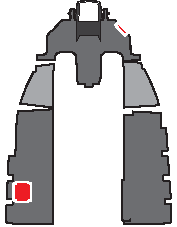
\includegraphics[width=\marginparwidth]{diagrams/cockpit/check_dbu.pdf}
        \caption{DBU Check}
    }
    \begin{enumerate}
        \item \textbf{DIGITAL BACKUP Switch} \dotfill \textbf{BACKUP}
        \begin{itemize}
            \item \textbf{DBU ON Light} --- \textbf{Illuminates}
        \end{itemize}
        \item Operate Controls --- check for normal control surface response
        \item \textbf{DIGITAL BACKUP Switch} \dotfill \textbf{OFF}
    \end{enumerate}
    \blueitem[Trim Check]
    \marginpar{
        \captionsetup{type=figure}
        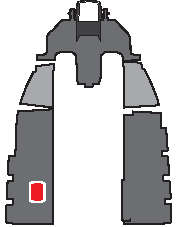
\includegraphics[width=\marginparwidth]{diagrams/cockpit/check_trim.pdf}
        \caption{Trim Check}
    }
    \begin{enumerate}
        \item \textbf{TRIM/AP DISC Swtich} \dotfill \textbf{DISC}
        \item \textbf{Stick Trim} \dotfill Activate in Pitch \& Roll
        \begin{itemize}
            \item No control surface motion 
            \item No TRIM wheel or indicator motion
        \end{itemize} 
        \item \textbf{TRIM/AP DISC Swtich} \dotfill \textbf{NORM}
        \item \textbf{Stick Trim} \dotfill Check \& Center
        \begin{itemize}
            \item Control surface motion 
            \item TRIM wheel motion
        \end{itemize} 
        \item \textbf{Yaw Trim Knob} \dotfill \textbf{Center}
    \end{enumerate}
\end{checklistenumerate}

\clearpage

\begin{checklistenumerate}[resume]
    \blueitem[MPO Check]
    \marginpar{
        \captionsetup{type=figure}
        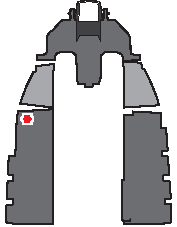
\includegraphics[width=\marginparwidth]{diagrams/cockpit/check_mpo.pdf}
        \caption{MPO Check}
    }
    \begin{enumerate}
        \item \textbf{Stick} \dotfill \textbf{Full Forward \& Hold}
        \item \textbf{MPO Switch} \dotfill \textbf{OVRD \& Hold}
        \begin{itemize}
            \item Horizontal Tail trailing edges move farther down
        \end{itemize} 
        \item \textbf{Stick \& MPO} \dotfill Release
    \end{enumerate}
    \blueitem[EPU Check]
    \marginpar{
        \captionsetup{type=figure}
        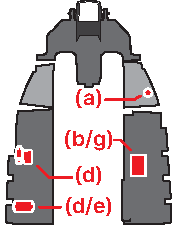
\includegraphics[width=\marginparwidth]{diagrams/cockpit/check_epu.pdf}
        \caption{EPU Check}
    }
    \begin{enumerate}
        \item \textbf{EPU FUEL Qty} \dotfill \textbf{95-102 Percent}
        \item \textbf{OXYGEN} \dotfill \textbf{100\%}
        \item \textbf{Throttle} \dotfill 10\% above \textbf{IDLE}
        \item \textbf{EPU/GEN TEST Switch} \dotfill \textbf{EPU/GEN \& Hold}
        \begin{itemize}
            \item \textbf{EPU AIR Light} --- \textbf{ON}
            \item \textbf{EPU GEN/PMG Lights} --- \textbf{OFF}
            \item \textbf{FLCS PWR Lights} --- \textbf{ON}
            \item \textbf{EPU Run Light} --- \textbf{ON} minimum 5s
        \end{itemize} 
        \item \textbf{EPU/GEN TEST Switch} \dotfill \textbf{OFF}
        \item \textbf{Throttle} \dotfill \textbf{IDLE}
        \item \textbf{OXYGEN} \dotfill \textbf{NORMAL}
    \end{enumerate}
\end{checklistenumerate}

\marginfigrestore